\section{Background}

In this section we present the background of NVMe interface and SPDK 
framework. We also present testFS, a user space file system that our 
file system is based on.

\subsection{NVMe and I/O Queue}

NVMe~\cite{nvme} is an open interface specification designed to allow host
software to communicate with a non-volatile memory subsystem (NVM) via a 
peripheral component interconnect express (PCIe) bus. Previous standards
such as serial-attacked SCSI and serial advanced technology attachment
can handle queue depths of 254 and 32 respectively. NVMe is able to 
handle queue depths of up to 65535 I/O queues with up to 64 Ki outstanding
commands per I/O queue, which allows an NVMe device to support parallel
operations. An I/O queue is composed of a submission queue and a completion
queue. Host software issues I/O commands to a submission queue and completions
are placed into the associated completion queue by the controller. Note that
the order of completions is not determined by the submission oder of the commands.

\subsection{SPDK and Block Devices}

SPDK~\cite{spdk} is an open source library that allows developer to implement
high performance, scalable, user-mode storage applications. A block device 
in SPDK is an abstraction of all block devices, where I/O commands are 
processed and issued to corresponding physical block devices such as NVMe 
devices and Malloc devices. SPDK provides a event framework, where  
different threads to exchange data through passing messages to one another.
It allows a user to build asynchronous, lockless, and high performance
applications.

\begin{figure}
  \centering
  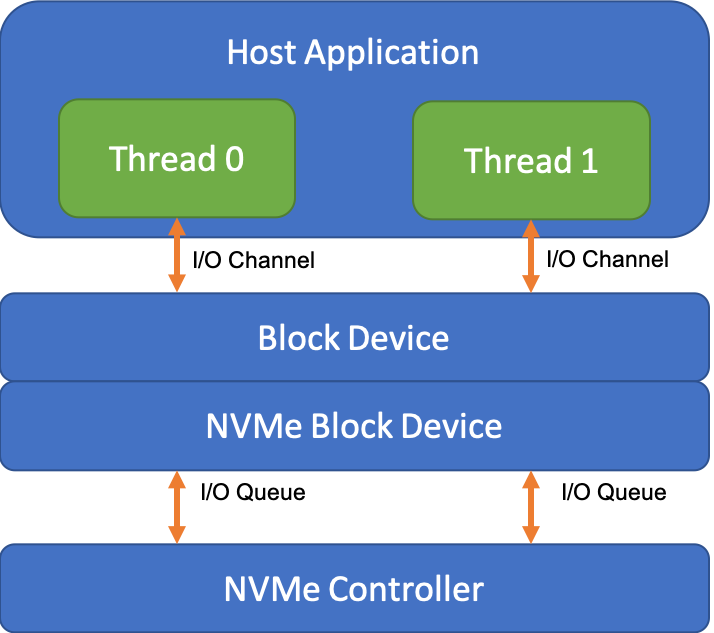
\includegraphics[height=6cm]{spdk_arch}
  \caption{Example of an SPDK application.}
  \label{fig:spdk_arch}
\end{figure}

For each thread, SPDK uses an io channel to represent the channel for accessing an 
I/O device. I/O requests issued to the block device will be forwarded to the underlying
physical device. In our implementation, io channel corresponds to I/O queue 
of the underlying NVMe device, the framework builds I/O commands based on I/O 
requests and submits them to submission queue. It then polls for I/O completion
on each queue pair with outstanding I/O to receive completion callbacks.  
Figure~\ref{fig:spdk_arch} provides a graphical
representation of a host application using SPDK block devices to interact with
an NVMe device. In the host application, each thread submit I/O requests to its
corresponding I/O channel and the I/O channel forward the I/O requests to the 
actual physical device based on the implementation of the physical block device.
The framework invokes the callback function when the I/O request is finished.

\subsection{TestFS}

TestFS\cite{testfs} is a user space file system which is similar to EXT3, a
journaled file system that is commonly used by the Linux kernel. TestFS
has three levels of indirections, which is illustrated in Figure~\ref{fig:testfs}.
A super block points to meta data and an inode block of the root directory. 
The meta data store the freemap of blocks as well as the checksum of the data blocks.
Inode blocks point to data blocks where the actual data are stored. In testFS, both 
directory data and indirect inode data are stored in data blocks. The
space for inode blocks and data blocks are pre-allocated and fixed during the
life cycle of testFS.

Note that our file system is based on testFS because testFS is well maintained, user
level, and well documented file system, that allows us to build a proof of concept
quickly. We believe our modifications to testFS can be applied to most of file systems.

\begin{figure}[h!]
  \centering
  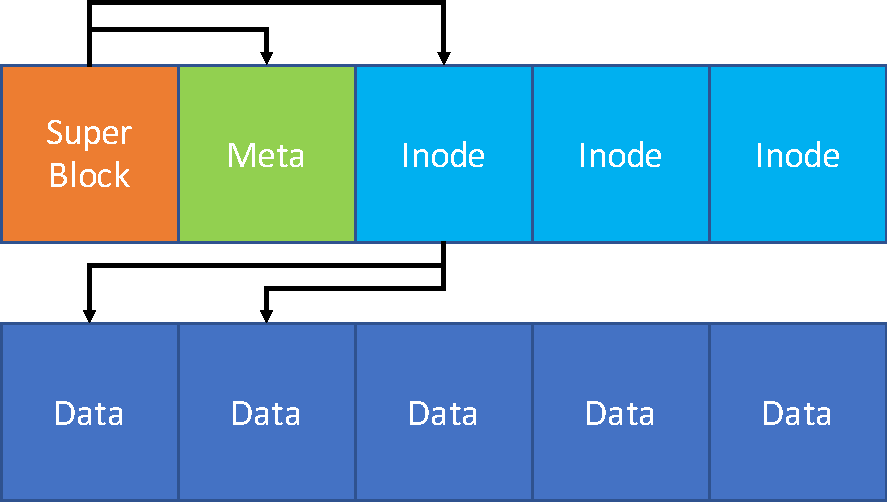
\includegraphics[height=3cm]{testfs}
  \caption{The layout of blocks with different types in testFS.}
  \label{fig:testfs}
\end{figure}
